\section{Confidential Computing (CC)}
\label{sec:confidential-computing}

Data can be in three distinct states: ``at rest'', ``in transit'', and ``in
use''. These three states describe data that are stored in persistent storage,
traversing a network, and data that is currently being processed. While
technologies protecting data ``at rest'' and ``in transit'' are commonly used
today, there are not many methods to protect data ``in use''.

By executing computations in hardware-based trusted execution environments
(TEEs) confidential computing protects data in use. In order to for a service
provider to be able to assure an application owner that the requested
environment can be trusted, remote attestation protocols (see Section
\ref{sec:remote-attestation}) are used.

The goal of confidential computing is to reduce the size of the trusted
computing base (TCB) of applications. The TCB of an application or system is the
set of all hardware, firmware, and software components that are critical to its
security.

\subsection{Trusted Execution Environments (TEEs)}
\label{sec:tee}

\subsubsection{Properties}

There are different definitions of a trusted execution environment (TEE) with
varying properties. The three main properties defined by the
\citeauthor{ccc2022technicalanalysis} \cite{ccc2022technicalanalysis} are:

\begin{description}
  \item[Data confidentiality]
    Prevent unauthorized entities to view data that is in use within a TEE.
  \item[Data integrity]
    Prevent unauthorized entities to add, remove, or change data while it is in
    use within a TEE.
  \item[Code integrity]
    Prevent unauthorized entities to add, remove, or change code executing in
    the TEE.
\end{description}

Combined, these three properties not only ensure the confidentiality of the data
but also allow clients to trust the results of a computation running inside a
TEE using the provided data.

TEEs often also provide evidence in the form of measurements of its initial
and/or current state. This evidence can then be verified by a remote party and
can help to decide whether to trust the TEE to provide the three properties
defined above. Typically, this evidence is cryptographically signed by hardware,
allowing the third party to verify the authenticity and integrity of the
evidence. This process is referred to as remote attestation, and we will look
the specifics of this process in Section \ref{sec:remote-attestation}.

\subsubsection{Hardware Support}

The security of a software layer can only be as strong as the layers below it.
This is why an ideal security solution acts from the lowest layer possible. By
providing security through the lowest layer -- the hardware -- it is possible to
remove all software layers between the hardware and the TEE from its TCB,
including system software such as the operating system or hypervisor. The only
component remaining in the TCB is the hardware providing the TEE properties.

Today most TEE implementations still rely on firmware components. This allows
manufacturers to more easily deploy bug fixes and security patches. While
firmware is still software, these TEE technologies provide hardware based
mechanisms that allow third parties to not only verify the trustworthiness of
the TEE, but also verify the configuration and integrity of the firmware and
software components involved in the creation and management of a TEE.

\subsubsection{Memory Protection}

Most TEE technologies today rely on the protection of memory in order to provide
the three properties defined above. They often provide two mechanisms,
protecting the confidentiality and integrity of data stored in memory:

\begin{description}
  \item[Memory Encryption]
    TEE technologies rely on a hardware component to encrypt data that is being
    transferred from the CPU to the physical memory of a machine and decrypt
    data moving from the memory to the CPU. Unlike homomorphic encryption, which
    provides specific computational functions directly on encrypted data
    \cite{monique2013homomorphicencryption}, TEE technologies transparently
    en-/decrypt data. Memory encryption strengthens the confidentiality of data
    in use, as untrusted software components that gain access to the memory of a
    TEE or malicious entities that have access to the physical memory of a
    machine, only see encrypted data.

  \item[Memory Access Control]
    On the other hand, memory integrity is guaranteed by enforcing that only the
    VM or process owning specific memory regions to be able to modify data
    stored in those. This is achieved by introducing new CPU instructions or a
    software component that enforces access control.
\end{description}

\subsection{TEE Models}
\label{sec:tee-models}

There are two distinct models of TEEs, process-based and VM-based.

\subsubsection{Process-based TEEs}
\label{sec:process-based-tees}

Process-based TEEs introduce a new programming model. A program needs to be
split into two components, trusted and untrusted. These are often referred to as
the ``enclave'' and ``host''. The enclave is executed in a TEE and as such
should contain all code that interacts with sensitive data, whereas the host
component is responsible for handling non-sensitive tasks like networking and
file I/O.

While the host is not shielded the enclave is protected from the rest of the
system, this includes

\begin{itemize}
  \item the enclave's own host
  \item other processes running on the same machine
  \item the operating system
  \item firmware such as the BIOS
  \item the hypervisor and host operating system (in virtualized environments)
  \item hardware other than the processor
\end{itemize}

Splitting a program into enclave and host is challenging. It requires a deep
understanding of security and how these process-based TEE solutions work. To
ease the development of such applications SDKs and frameworks often hide the
split between host and enclave from the developer \cite{schuster2022}.

Library OSes like Gramine and Occlum go even further and provide a POSIX-like
runtime environment with support for network, file I/O, and multithreading.
Because applications running inside the enclave do not have access to the
underlying OS, library OSes provide libraries that implement OS system calls in
form of library functions. These libraries then interface with a boilerplate
host for I/O \cite{tsai2014graphene}.

Even though these SKDs, frameworks, and library OSes ease the development and
make porting of existing applications easier, using process-based TEEs still
requires more development effort and more often then not modifications of
existing applications.

\subsubsection{VM-based TEEs}
\label{sec:vm-based-tees}

The main concept of VM-based TEEs is to apply the TEE properties to a full
virtual machine. While traditional VMs can share memory with the hypervisor in
order to support communication between VMs or with the hypervisor, the memory of
VM-based TEEs are not accessible by the hypervisor.

While this model allows running basically any application without modifications,
this model has a much larger TCB compared to the process-based TEE model.
VM-based TEEs however are still specifically designed to remove the following
components from the VMs TCB:

\begin{itemize}
  \item VM firmware (e.g. OVMF)
  \item the hypervisor and host operating system
  \item hardware other than the processor
\end{itemize}

\subsubsection{Comparison}

\begin{figure}[H]
  \centering
  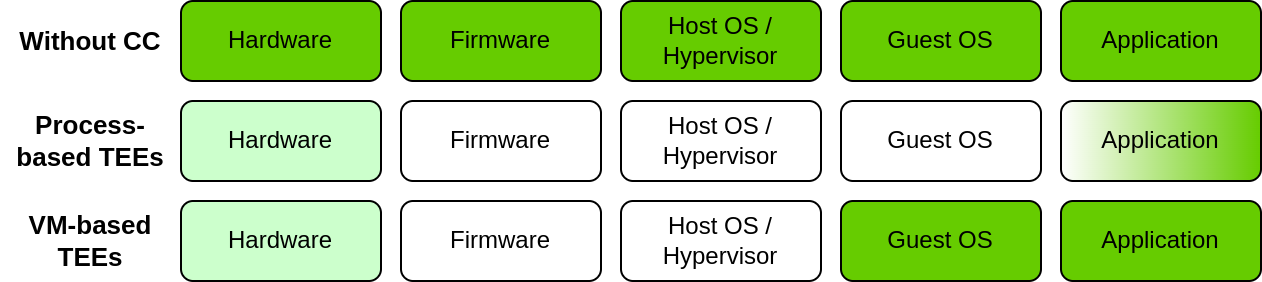
\includegraphics[width=\linewidth]{resources/tee-models-comparison.drawio.png}
  \caption{Comparison of trusted execution environment models in a virtualized environment.}
  \label{figure:cc-tee-comparison}
\end{figure}

Figure \ref{figure:cc-tee-comparison} shows a simplified comparison between the
TCBs of an application running without confidential computing, inside a
process-based TEE, and inside a VM-based TEE. In both TEE models a hardware
component enforces the TEE properties and thus the hardware has to be partly
trusted. The main difference between the two models is the size of the TCB,
where process-based TEEs only have a small trusted component of the application
(the enclave), the whole VM is trusted in a VM-based TEE.

\subsection{Commercially Available TEE Technologies}
\label{sec:commercial-tee-technologies}

\begin{description}
  \item[Intel SGX]
    Intel Software Guard Extensions (SGX) provides process-based TEEs by relying
    on hardware to establish enclaves that contain application code and
    confidential data. As the name implies, it is an extension of Intel's CPU
    instruction set architecture \cite{costan2016sgx}.

    The CPU protects a designated memory area called the Processor Reserved
    Memory (PRM) established by SGX, by ensuring that other software, such as
    the system software (hypervisor or OS) and DMA devices do not have access to
    the PRM. Confidential data and code of enclaves is stored in the Enclave
    Page Cache (EPC), which is a subset of the PRM. SGX relies on an untrusted
    system software to manage EPC pages by assigning EPC pages to enclaves and
    evicting these pages if needed. However, system software cannot directly
    access the EPC and the CPU maintains Enclave Page Cache Map (EPCM) in the
    EPC that keeps track of allocated EPC pages and the enclave which owns the
    page. Using the EPCM the CPU checks the correctness of the system software's
    allocation decisions, ensures that a EPC page is only assigned to a single
    enclave, and that only the assigned enclave can access and modify the EPC
    page. The CPU also encrypts EPC pages while they are stored in physical
    memory in order to prevent leaking confidential data through PME attacks and
    guaranteeing confidentiality of EPC pages after eviction.

    Initially, the system software ask the CPU to copy data from unprotected
    memory into EPC pages and assigns the pages to the enclave. After the EPC
    pages are loaded, the enclave is marked as initialized and the system
    software can not access nor modify EPC pages anymore. The CPU then measures
    SGX components and the initial EPC pages of the enclave, producing an
    attestation report which is then signed by the CPU. The signature can
    subsequently be used to verify the authenticity of the measurements, and the
    measurements to verify the integrity of the enclave.

  \item[AMD SEV]
    AMD SEV-SNP is the latest iteration of AMD's Secure Encrypted Virtualization
    (SEV) technology \cite{amd2021sev, amd2017seves, amd2020sevsnp} and as the
    name implies provides VM-based TEEs.

    SEV relies on hardware embedded encryption engines that encrypt or decrypt
    memory pages written to or read from the physical memory of a machine. It
    utilizes the AMD Secure Processor (AMD-SP), which is integrated into the
    same chip as the CPU, to generate and manage cryptographic keys used for the
    en-/decryption. All software and data is tagged with an Address Space
    Identifier (ASID). The CPU uses the ASID to restrict the usage of data to
    the owner with the same ASID and protect the data from any unauthorized
    usage inside the CPU. However, in the first iteration of SEV the registers
    of a vCPU could be used to leak confidential data when shutting down a VM.
    Subsequently, AMD released their second iteration SEV-ES (Encrypted State),
    which not only encrypted VM memory but also the vCPU's registers. The latest
    version SEV-SNP (Secure Nested Paging) introduced further features in order
    to protect the integrity of VM memory.

    The attestation process for SEV VMs is similar to the attestation process of
    SGX enclaves. A hypervisor launches a VM and after the VM is fully loaded
    the VM's memory is encrypted. After which the AMD-SP measures SEV components
    and VM memory pages and signs these measurements. Again, the signature can
    then be used for verifying the authenticity of the measurements, and the
    measurements to verify the integrity of the VM. Attestation support in SEV
    and SEV-ES was limited, as measurements could only be requested during the
    launch of a VM. SEV-SNP supports the request of measurements at any time,
    enabling more flexible attestation.
\end{description}

As TEE technologies widely differ in their implementations and TEE model they
offer, following this section we will treat the hardware and software components
that create and protect TEEs as a single platform, which consists of all
hardware and software components relevant in the TEE create and protection
process, and refer to it as the ``TEE platform''.

\subsection{Limitations}
\label{sec:limitations}

\begin{description}
  \item[Performance Impact]
    Generally, currently existing solutions either require careful configuration
    in order to achieve acceptable performance or are inappropriate for specific
    types of workloads (e.g. high performance computing)
    \cite{akram2021performance}.
  \item[CPU centric focus]
    Most of today's CC solutions focus on a CPU-level view of memory
    permissions. This limits the application of CC to heterogeneous computing
    systems, where heterogeneous accelerators are used in order to speed up
    specific computations (e.g. NPUs for machine learning workloads
    \cite{chen2014mlaccelerators}). However, there is ongoing work on
    integrating CC into heterogeneous computing systems \cite{jiang2022cronus}.
  \item[New technology that requires further research]
    Since the introduction of Intel SGX in 2015 numerous vulnerabilities found
    in the SGX architecture \cite{fei2021sgxvulnerabilities}. AMD SEV has also
    not been spared, which until now required two iterations to fix the issues
    that have been discovered. Both technologies also depend on existing
    software such as hypervisors, VM firmware, and operating systems to
    implement the integration of these technologies. These implementations also
    require further research and testing in order to find vulnerabilities and
    security issues in their designs.
\end{description}
